
\documentclass[ucs]{beamer}

\usetheme{GSyC}
%\usebackgroundtemplate{\includegraphics[width=\paperwidth]{gsyc-bg.png}}


\usepackage[spanish]{babel}   
\usepackage[utf8x]{inputenc}
\usepackage{graphicx}
\usepackage{amssymb} % Simbolos matematicos
\usepackage{lmodern,textcomp}  % para usar el carácter € tal cual



% Metadatos del PDF, por defecto en blanco, pdftitle no parece funcionar
   \hypersetup{%
     pdftitle={Cascading Style Sheets},
     %pdfsubject={Diseño y Administración de Sistemas y Redes},%
     pdfauthor={GSyC},%
     pdfkeywords={},%
   }
%


% Para colocar un logo en la esquina inferior de todas las transpas
%   \pgfdeclareimage[height=0.5cm]{gsyc-logo}{gsyc}
%   \logo{\pgfuseimage{gsyc-logo}}


% Para colocar antes de cada sección una página de recuerdo de índice
%\AtBeginSection[]{
%  \begin{frame}<beamer>{Contenidos}
%    \tableofcontents[currentframetitle]
%  \end{frame}
%}



\begin{document}

% Entre corchetes como argumento opcional un título o autor abreviado
% para los pies de transpa
\title[CSS]{CSS: Cascading Style Sheets}
%\subtitle{Diseño y Administración de Sistemas y Redes}
\author[GSyC]{Escuela Técnica Superior de Ingeniería de Telecomunicación\\
Universidad Rey Juan Carlos}
\institute{gsyc-profes (arroba) gsyc.urjc.es}
\date[2017]{Octubre de 2017}


%% TÍTULO
\begin{frame}
  \titlepage
  % Oportunidad para poner otro logo si se usó la opción nologo
  % \includegraphics[width=2cm]{logoesp}  
\end{frame}



%% LICENCIA DE REDISTRIBUCIÓN DE LAS TRANSPAS
%% Nota: la opción b al frame le dice que justifique el texto
%% abajo (por defecto c: centrado)
\begin{frame}[b]



\vspace{1cm}
\begin{footnotesize}

\begin{flushright}
Las transparencias del tema ``CSS - Hojas de estilo'' \\
están basadas en el libro de librosweb.es \\
disponible en http://www.librosweb.es/css/ \\
Se ha pedido explícitamente autorización al autor original \\
para realizar esta obra derivada con fines educativos.

\copyright Javier Eguiluz - Librosweb.es \\
\vspace{1cm}
\end{flushright}



\begin{flushright}
{


Derivado a partir de material de \\
Jesús M. González-Barahona y Gregorio Robles.

El original está disponible en \\
\url{http://cursosweb.github.io}\\
  Algunos derechos reservados. \\
  Este trabajo se distribuye bajo la licencia \\
  Creative Commons Attribution Share-Alike 4.0\\
}


\end{flushright}  


\end{footnotesize}
\end{frame}



%% ÍNDICE
%\begin{frame}
%  \frametitle{Contenidos}
%  \tableofcontents
%\end{frame}




\section{Hojas de estilo CSS}


%%---------------------------------------------------------------

\begin{frame}
\frametitle{¿Qué es CSS?}

\begin{itemize}
  \item CSS, \emph{Cascading Style Sheets} es un lenguaje de hojas de estilos creado para {\bf controlar el aspecto} o presentación de los documentos electrónicos definidos con HTML
  \item Es la mejor forma de {\bf separar los contenidos y su presentación} y es imprescindible para crear páginas web complejas
  \begin{itemize}
    \item Obliga a crear documentos HTML bien definidos y con significado completo (también llamados \emph{documentos semánticos})
    \item Mejora la accesibilidad del documento
    \item Reduce la complejidad de su mantenimiento
    \item Permite visualizar el mismo documento en infinidad de dispositivos diferentes
  \end{itemize}
\end{itemize}

\end{frame}

%%---------------------------------------------------------------

\begin{frame}[fragile]
\frametitle{Antes del CSS}

{\footnotesize
\begin{verbatim}
<!DOCTYPE html>
<html>
<head>
 <meta http-equiv="Content-Type" content="text/html; charset=iso-8859-1"/>
 <title>Ejemplo de estilos sin CSS</title>
</head>
 
<body>
 <h1><font color="red" face="Arial" size="5">
    Titular de la página
 </font></h1>
 <p><font color="gray" face="Verdana" size="2">
   Un párrafo de texto no muy largo.
 </font></p>
</body>
</html>
\end{verbatim}
}

\end{frame}

%%---------------------------------------------------------------

\begin{frame}[fragile]
\frametitle{Con CSS}

{\footnotesize
\begin{verbatim}
<!DOCTYPE html>
<html>
<head>
  <meta charset="utf-8">
  <title>Ejemplo de estilos con CSS</title>
  <style>
    h1 { color: red;  font-family: Arial;   font-size: large;  }
    p  { color: gray; font-family: Verdana; font-size: medium; }
  </style>
</head>
 
<body>
  <h1>Titular de la página</h1>
  <p>Un párrafo de texto no muy largo.</p>
</body>
</html>
\end{verbatim}
}

\end{frame}

%%---------------------------------------------------------------

\begin{frame}
\frametitle{CSS en un documento HTML}

Se pueden integrar instrucciones CSS de varias maneras en un documento
HTML:

\begin{enumerate}
  \item Incluir CSS en el mismo documento HTML
  \item Definir CSS en un archivo externo
  \item Incluir CSS en los elementos HTML
\end{enumerate}

\end{frame}

%%---------------------------------------------------------------

\begin{frame}
\frametitle{Glosario Básico (I)}

\begin{center}
\begin{figure}[p]
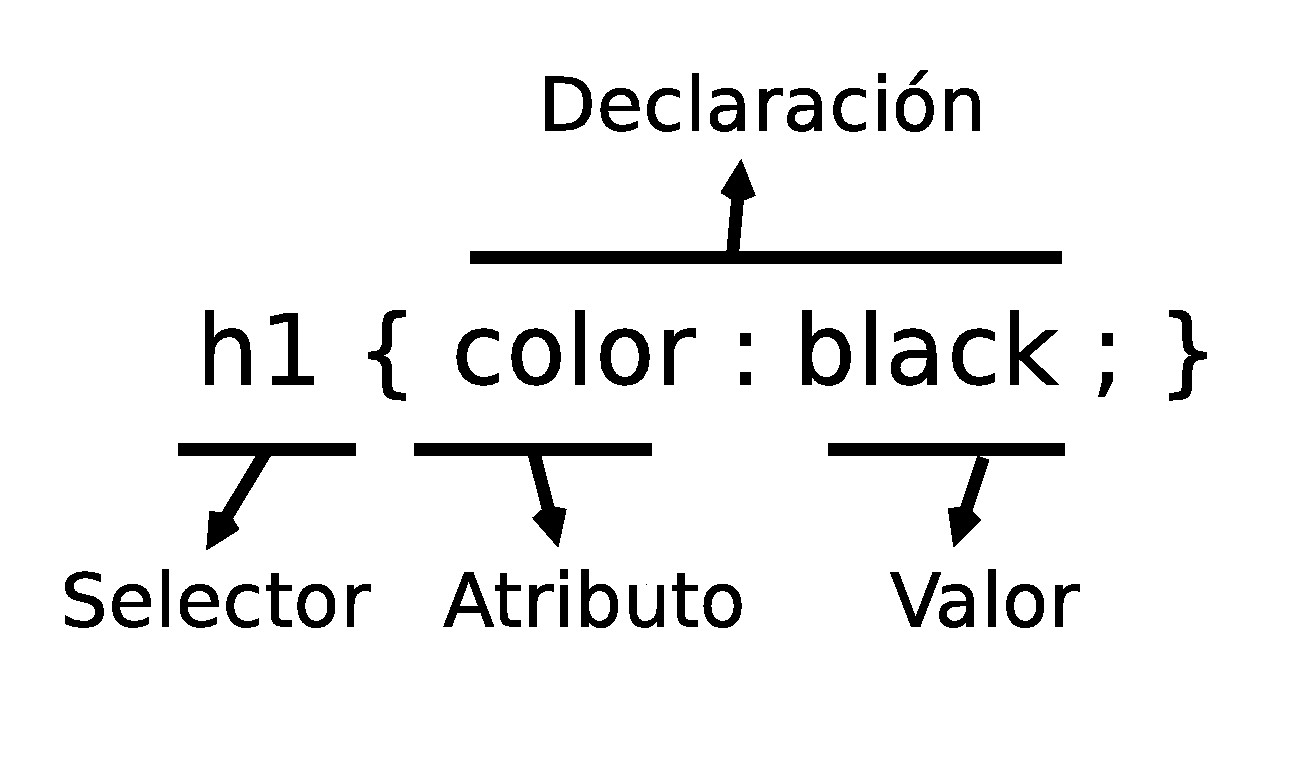
\includegraphics[width=0.6\textwidth]{figs/f0101_miguel}
\end{figure}
\end{center}

\begin{itemize}
  \item {\bf Regla}: cada uno de los estilos que componen una hoja de estilos CSS. Cada regla está compuesta de una parte de ``selectores'', un símbolo de ``llave de apertura'' (\{), otra parte denominada ``declaración'' y por último, un símbolo de ``llave de cierre'' (\}).
  \item {\bf Selector}: indica el elemento o elementos HTML a los que se aplica la regla CSS.
\end{itemize}

\end{frame}

%%---------------------------------------------------------------

\begin{frame}
\frametitle{Glosario Básico (y II)}

\begin{center}
\begin{figure}[p]
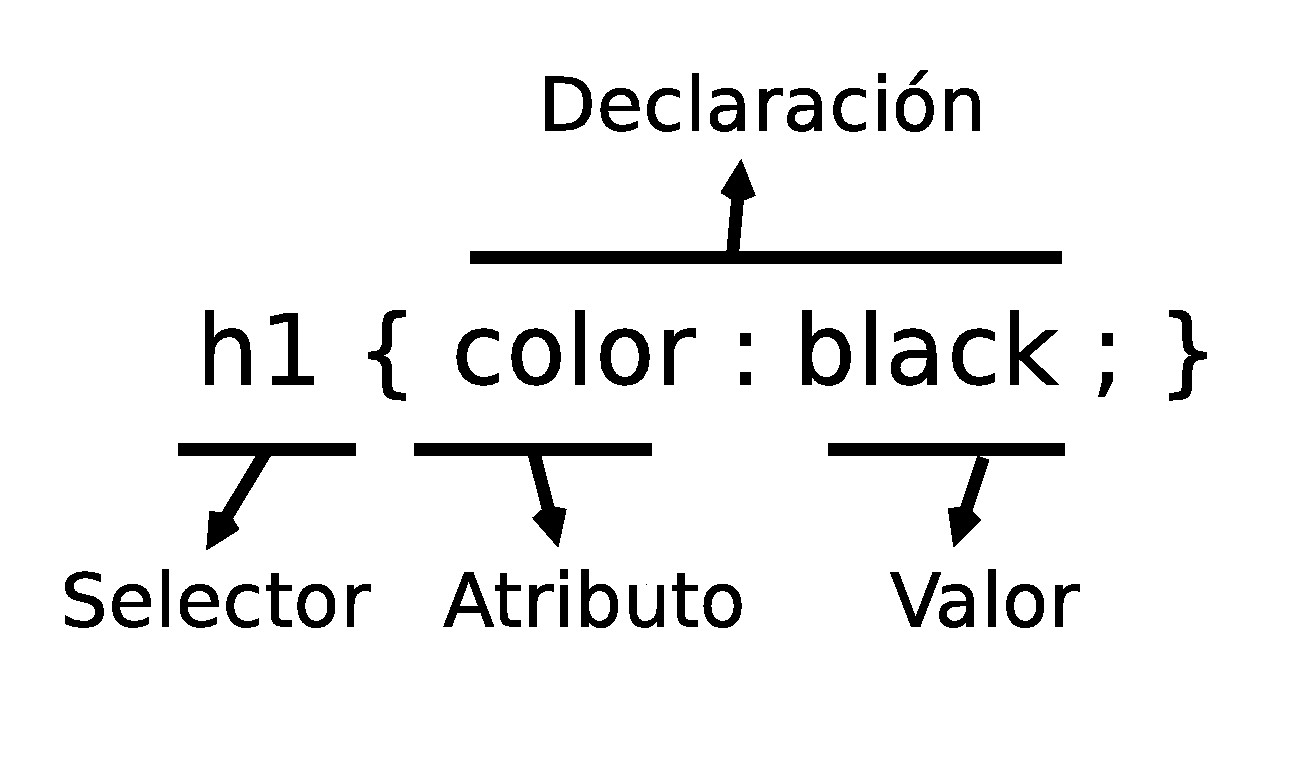
\includegraphics[width=0.52\textwidth]{figs/f0101_miguel}
\end{figure}
\end{center}

\begin{itemize}
  \item {\bf Declaración}: especifica los estilos que se aplican a los elementos. Está compuesta por una o más atributos CSS.
  \item {\bf Atributo}: característica que se modifica en el elemento seleccionado, como por ejemplo su tamaño de letra, su color de fondo, etc.
  \item {\bf Valor}: establece el nuevo valor de la característica modificada en el elemento.
\end{itemize}

CSS 2.1 define 115 atributos, mientras que CSS 3 define 239 atributos.

\end{frame}

%%---------------------------------------------------------------
%
%\begin{frame}
%\frametitle{Sintaxis}
%
%\begin{itemize}
%  \item Sucesión de palabras sin ningún carácter que las separe (paréntesis, comas, barras, etc.) el valor del atributo se debe indicar tal y como se muestra y con esas palabras en el mismo orden.
%  \item Sucesión de valores separados por una barra simple el valor del atributo debe tomar uno y sólo uno de los valores indicados
%  \item Sucesión de valores separados por una barra doble el valor del atributo puede tomar uno o más valores de los indicados y en cualquier orden.
%  \item Cada valor o agrupación de valores se puede indicar el tipo de valor: opcional, obligatorio, múltiple o restringido.
%  \item Más: * = cero o más veces; + = una o más veces; ? = opcional; {n1, n2} = entre n1 y n2 veces
%\end{itemize}
%
%\end{frame}


%%---------------------------------------------------------------

\subsubsection*{Selectores}

\begin{frame}
\frametitle{Selectores}

\begin{itemize}
  \item A un mismo elemento HTML se le pueden aplicar varias reglas 
  \item Cada regla puede aplicarse a un número ilimitado de elementos
  \item Cuando el selector de dos o más reglas CSS es idéntico, se pueden agrupar las declaraciones de las reglas para hacer las hojas de estilos más eficientes
  \item Cuando se establece el valor de un atributo CSS en un elemento, sus elementos descendientes heredan de forma automática el valor de ese atributo
\end{itemize}



\end{frame}

%%----------------------------------------------
\begin{frame}[fragile]


    \begin{itemize}
    \item
CSS 2.1 incluye una docena de tipos diferentes de selectores, que permiten seleccionar de forma muy precisa elementos individuales o conjuntos de elementos dentro de una página web.

    \item
Los selectores de CSS tienen mucha utilidad porque también son usados en JQuery
    \end{itemize}
\end{frame}

%%---------------------------------------------------------------

\begin{frame}
\frametitle{Selectores básicos}

\begin{enumerate}
  \item Selector universal
  \item Selector de tipo o etiqueta
  \item Selector descendente
  \item Selector de clase
  \item Selector de identidad
\end{enumerate}

\end{frame}

%%---------------------------------------------------------------

\begin{frame}[fragile]
\frametitle{Selector Universal}

\begin{itemize}
  \item No se utiliza habitualmente
  \item Generalmente es equivalente para poner estilo a $<body>$
  \item Se suele combinar con otros selectores y además, forma parte de algunos hacks muy utilizados
\end{itemize}

\begin{verbatim}
* {
  margin: 0;
  padding: 0;
}
\end{verbatim}

\end{frame}

%%---------------------------------------------------------------

\begin{frame}[fragile]
\frametitle{Selector de tipo o etiqueta}

\begin{itemize}
  \item Selecciona todos los elementos de la página cuya etiqueta HTML coincide con el valor del selector
  \item Se pueden agrupar todas las reglas individuales en una sola regla con un selector múltiple.
  \item Buena práctica: agrupar los atributos comunes de varios elementos en una única regla CSS y posteriormente definir los atributos específicos de esos mismos elementos
\end{itemize}

{\footnotesize
\begin{verbatim}
h1, h2, h3 {
  color: #8A8E27;
  font-weight: normal;
  font-family: Arial, Helvetica, sans-serif;
}
 
h1 { font-size: 2em; }
h2 { font-size: 1.5em; }
h3 { font-size: 1.2em; }
\end{verbatim}
}

\end{frame}

%%---------------------------------------------------------------

\begin{frame}[fragile]
\frametitle{Selector descendente}

\begin{itemize}
  \item Selecciona los elementos contenidos dentro de otros elementos. 
\end{itemize}
Ejemplo: elementos span contenidos dentro de elementos p


  \begin{footnotesize}
  \begin{verbatim}
p span { color: red; }
[...]
<p>
  ...
  <span>Texto1</span>
  <a href="">...<span>Texto2</span></a>
  ...
</p>
  \end{verbatim}
  \end{footnotesize}

Texto 1 evidentemente cumple la regla. 

Texto 2 es un elemento span contenido dentro de un enlace contenido dentro de un elemento
p.
Por tanto, Texto 2 están contenido dentro de un p.
Aunque no sea descendente directo, es descendente y la regla se aplica.

\end{frame}

%%---------------------------------------------------------------

\begin{frame}
\frametitle{Ejercicio}

¿Qué elementos se seleccionarían con estos tipos de selectores?

\begin{itemize}
  \item p a span em \{ text-decoration: underline; \}
  \item p, a, span, em \{ text-decoration: underline; \}
  \item p a \{ color: red; \}
  \item p * a \{ color: red; \}
\end{itemize}

\end{frame}

%%---------------------------------------------------------------

\begin{frame}[fragile]
\frametitle{Selector de clase}

\begin{itemize}
  \item Se utiliza el atributo class de HTML sobre ese elemento para indicar directamente la regla CSS que se le debe aplicar
  \item Se crea en el archivo CSS una nueva regla llamada destacado con todos los estilos que se van a aplicar al elemento
  \item Se prefija el valor del atributo class con un punto (.)
\end{itemize}


  \begin{footnotesize}
  \begin{verbatim}
  .destacado { color: red; }
  [...]
  <p class="destacado">
    Lorem ipsum dolor sit amet...
  </p>
  <p>Nunc sed lacus et
    <a href="#" class="destacado">est adipiscing</a>
  </p>
  <p>Class aptent taciti <em class="destacado">sociosqu ad</em>
  </p>
  \end{verbatim}
  \end{footnotesize}

Esta regla se aplica a cualquier elemento de clase \emph{destacado}



\end{frame}

%%---------------------------------------------------------------

\begin{frame}[fragile]
\frametitle{Selector de clase más específico}

\begin{itemize}
  \item Combinando el selector de tipo y el selector de clase, se obtiene un selector mucho más específico.
\end{itemize}

{\footnotesize
\begin{verbatim}
  p.destacado { color: red }
  [...]
  <p class="destacado">
    Lorem ipsum dolor sit amet...
  </p>
  <p>Nunc sed lacus et
    <a href="#" class="destacado">est adipiscing</a>
  </p>
  <p>Class aptent taciti <em class="destacado">sociosqu ad</em>
  </p>
\end{verbatim}
}

Esta regla se aplica a los elementos de tipo párrafo, que además sean
de clase \emph{destacado}. (En este ejemplo, solo una vez)
\end{frame}

%%---------------------------------------------------------------

\begin{frame}
\frametitle{Ejercicio}

¿Qué elementos se seleccionarían con estos tipos de selectores?

\begin{itemize}
  \item p.aviso \{ ... \}
  \item p .aviso \{ ... \}
  \item p, .aviso \{ ... \}
  \item *.aviso \{ ... \}
\end{itemize}

\end{frame}

%%---------------------------------------------------------------

\begin{frame}[fragile]
\frametitle{Selectores de identificador}

\begin{itemize}
  \item Aplica estilos CSS a un único elemento de la página
  \item El valor del atributo id no se puede repetir en dos elementos diferentes de una misma página
\end{itemize}

\begin{verbatim}
#destacado { color: red; }
 
<p>Primer párrafo</p>
<p id="destacado">Segundo párrafo</p>
<p>Tercer párrafo</p>
\end{verbatim}

\end{frame}


%%---------------------------------------------------------------

\begin{frame}
\frametitle{Ejercicio}

¿Qué elementos se seleccionarían con estos tipos de selectores?

\begin{itemize}
  \item p\#aviso \{ ... \}
  \item p \#aviso \{ ... \}
  \item p, \#aviso \{ ... \}
  \item *\#aviso \{ ... \}
\end{itemize}


\end{frame}

%%---------------------------------------------------------------

\begin{frame}
\frametitle{Ejercicio: Combinación de selectores}

¿Qué elementos se seleccionarían con estos tipos de selectores?

\begin{itemize}
  \item .aviso .especial \{ ... \}
  \item div.aviso span.especial \{ ... \}
  \item ul\#menuPrincipal li.destacado a\#inicio \{ ... \}
\end{itemize}

\end{frame}

%%---------------------------------------------------------------

\begin{frame}
\frametitle{Colisión de estilos (simplificado)}

\begin{enumerate}
  \item Cuanto más específico sea un selector, más importancia tiene su regla asociada.
  \item A igual especificidad, se considera la última regla indicada.
\end{enumerate}

\end{frame}



%%---------------------------------------------------------------
\begin{frame}[fragile]
\frametitle{Otros selectores}
\begin{itemize}
\item
Concatenación de clases

\verb|.clase1.clase2 {atributo:valor;}|


La regla se aplica a los elementos cuyo atributo
\emph{class}
contengan tanto
\emph{clase1}
como
\emph{clase2}

\item
Selector hijo directo

\verb|p > span {atributo:valor;}|

Elementos span directamente contendidos dentro de un elemento p

\item
Selector adayacente

\verb|h2 + h3 {atributo:valor;}|

Elemento h3 inmediatamente después de un elemento h2

\end{itemize}

\end{frame}




%%---------------------------------------------------------------
\begin{frame}[fragile]
\frametitle{Selector de atributos}
\begin{itemize}
\item
\verb|div[class] { atributo: valor;}|

Elementos div que tengan establecido un atributo con nombre \emph{class}


\item
\verb|div[class="nacional"] { atributo: valor;}|

Elementos div que tengan establecido un atributo con nombre \emph{class} y valor
\emph{nacional}

\item
\verb|div[class~="nacional"] { atributo: valor;}|

Elementos div que tengan establecido un atributo con nombre \emph{class} y al 
menos uno de sus valores sea
\emph{nacional}


\end{itemize}


\end{frame}




%%---------------------------------------------------------------

\subsubsection*{Unidades y colores}

\begin{frame}
\frametitle{Unidades de medida}

\begin{itemize}
  \item Unidades absolutas
  \begin{itemize}
    \item in, cm, mm, pt, pc
  \end{itemize}
  \item Unidades relativas
  \begin{itemize}
    \item em, ex, px
  \end{itemize}
  \item Porcentajes
\end{itemize}

En general, se recomienda el uso de unidades relativas siempre que sea posible

Normalmente se utilizan píxel y porcentajes para definir el layout del documento (básicamente, la anchura de las columnas y de los elementos de las páginas) y em y porcentajes para el tamaño de letra de los textos.

\end{frame}

%%---------------------------------------------------------------

\begin{frame}
\frametitle{Especificación del color}
Hay dos formas principales de indicar el color

\begin{itemize}
\item 
Mediante su nombre

Los 18 principales son:

red, cyan, blue, darkblue, lightblue, purple, yellow,
lime, magenta, white, silver, gray/grey, black,
orange, brown, maroon, green, olive

  \item 
Mediante su código hexadecimal

Se representa por con una almohadilla y 6 dígitos hexadecimales
(dos dígitos para el rojo,
dos dígitos para el verde y 
dos dígitos para el azul)

Ejemplos:

\begin{flushleft}
\begin{figure}[p]
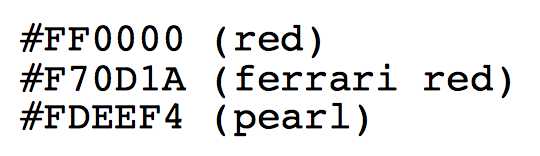
\includegraphics[width=0.37\textwidth]{figs/colores}
\end{figure}
\end{flushleft}

\end{itemize}

\end{frame}



%%---------------------------------------------------------------
\begin{frame}[fragile]
\frametitle{}
Los principales atributos relacionados con el color son
\begin{itemize}
\item
color

\item
backgroud-color

\item
border-color

\end{itemize}

\end{frame}





%%---------------------------------------------------------------
\begin{frame}[fragile]
\frametitle{Atributos relacionados con el texto}
\begin{itemize}
\item
Alineación

  \begin{footnotesize}
  \begin{verbatim}
text-align: left | right | center | justify | initial | inherit;
  \end{verbatim}
  \end{footnotesize}

\item
Subrayado


  \begin{footnotesize}
  \begin{verbatim}
text-decoration: none | underline | overline | line-through |
                 initial | inherit;
  \end{verbatim}
  \end{footnotesize}



\item
Tamaño

  \begin{footnotesize}
  \begin{verbatim}
font-size: medium | xx-small | x-small | small | large | 
           x-large | xx-large | smaller | larger | (length) |
           initial | inherit;
  \end{verbatim}
  \end{footnotesize}


\item
Estilo

  \begin{footnotesize}
  \begin{verbatim}
font-style: normal | italic | oblique | initial | inherit;

  \end{verbatim}
  \end{footnotesize}



\end{itemize}

\end{frame}



%%---------------------------------------------------------------
\begin{frame}[fragile]
\frametitle{Atributos relacionados con los bordes}


Los atributos del borde de una caja se especifican con:

    \begin{itemize}
    \item
border-width

    \item
border-style

    \item
border-color
    \end{itemize}

Puede abreviarse como simplemente \emph{border}



\begin{itemize}
\item
Ancho del borde


  \begin{footnotesize}
  \begin{verbatim}
border-width: medium | thin | thick | (length) | 
              initial | inherit;
  \end{verbatim}
  \end{footnotesize}


\item
Estilo del borde

  \begin{footnotesize}
  \begin{verbatim}
border-style: none | hidden | dotted | dashed | solid | double |
              groove | ridge | inset | outset | initial | inherit;
  \end{verbatim}
  \end{footnotesize}



\end{itemize}

\end{frame}





%%---------------------------------------------------------------

\begin{frame}
\frametitle{Tipos de elementos (I)}

El estándar HTML clasifica a todos sus elementos en dos grandes grupos:

Elementos de línea:

\begin{itemize}
  \item Los elementos en línea (``inline elements'' en inglés) no empiezan necesariamente en nueva línea y sólo ocupan el espacio necesario para mostrar sus contenidos.

\end{itemize}

\end{frame}

%%---------------------------------------------------------------

\begin{frame}
\frametitle{Tipos de elementos (II)}

Elementos de bloque:

\begin{itemize}
  \item Los elementos de bloque (``block elements'' en inglés) siempre empiezan en una nueva línea y ocupan todo el espacio disponible hasta el final de la línea
\end{itemize}

\begin{center}
\begin{figure}[p]
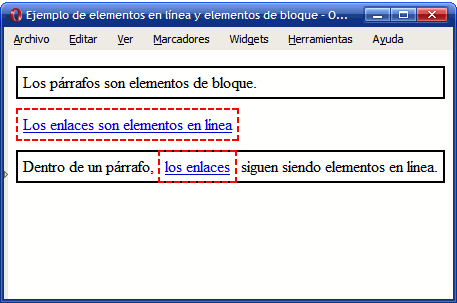
\includegraphics[width=0.8\textwidth]{figs/f0501.png}
\end{figure}
\end{center}

Por sus características, los elementos de bloque no pueden insertarse dentro de elementos en línea y tan sólo pueden aparecer dentro de otros elementos de bloque. En cambio, un elemento en línea puede aparecer tanto dentro de un elemento de bloque como dentro de otro elemento en línea.

\end{frame}



%%---------------------------------------------------------------

\subsubsection*{El Modelo de Cajas}

\begin{frame}
\frametitle{El modelo de cajas}

\begin{itemize}
  \item Es el comportamiento de CSS que hace que todos los elementos de las páginas se representen mediante cajas rectangulares
  \item  Cada vez que se inserta una etiqueta HTML, se crea una nueva caja rectangular que encierra los contenidos de ese elemento
\end{itemize}


\begin{center}
\begin{figure}[p]
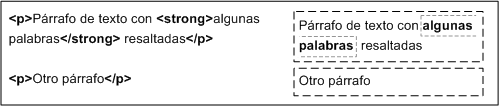
\includegraphics[width=0.8\textwidth]{figs/f0402.png}
\end{figure}
\end{center}

\end{frame}

%%---------------------------------------------------------------

\begin{frame}
\frametitle{El modelo de cajas (II)}

\begin{itemize}
  \item No son visibles a simple vista porque inicialmente no muestran ningún color de fondo ni ningún borde
\end{itemize}

\begin{center}
\begin{figure}[p]
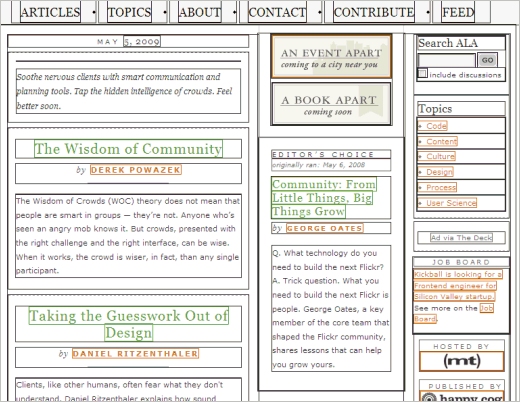
\includegraphics[width=0.55\textwidth]{figs/f0401.png}
\end{figure}
\end{center}
{\footnotesize
Ejemplo de http://www.alistapart.com/ después de forzar a que todas las cajas muestren su borde
}

\end{frame}

%%---------------------------------------------------------------

\begin{frame}
\frametitle{El modelo de cajas (III)}

\begin{itemize}
  \item Los navegadores crean y colocan las cajas de forma automática, pero CSS permite modificar todas sus características. Cada una de las cajas está formada por seis partes, tal y como muestra la siguiente imagen:
\end{itemize}


\begin{center}
\begin{figure}[p]
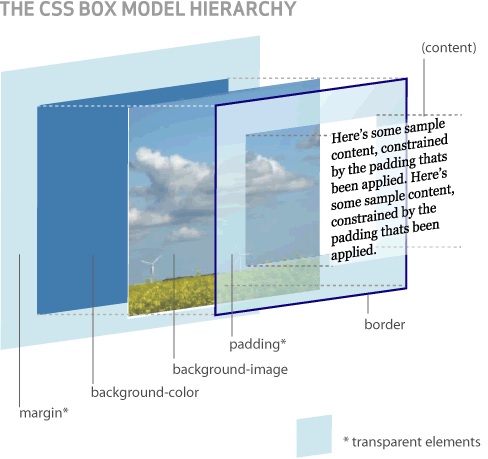
\includegraphics[width=0.45\textwidth]{figs/f0403.png}
\end{figure}
\end{center}
{\footnotesize
(Esquema utilizado con permiso de http://www.hicksdesign.co.uk/boxmodel/)
}
\end{frame}

%%---------------------------------------------------------------

\begin{frame}
\frametitle{Partes que componen cada caja}

\begin{itemize}
  \item {\bf Contenido} (content): se trata del contenido HTML del elemento (las palabras de un párrafo, una imagen, el texto de una lista de elementos, etc.)
  \item {\bf Relleno} (padding): espacio libre opcional existente entre el contenido y el borde.
  \item {\bf Borde} (border): línea que encierra completamente el contenido y su relleno.
  \item {\bf Imagen de fondo} (background image): imagen que se muestra por detrás del contenido y el espacio de relleno.
  \item {\bf Color de fondo} (background color): color que se muestra por detrás del contenido y el espacio de relleno.
  \item {\bf Margen} (margin): separación opcional existente entre la caja y el resto de cajas adyacentes.
\end{itemize}

\end{frame}


%%---------------------------------------------------------------

\begin{frame}[fragile]
\frametitle{Margen, relleno, bordes y modelo de cajas (I)}

\begin{itemize}
  \item El margen, el relleno y los bordes establecidos a un elemento determinan la anchura y altura final del elemento
\end{itemize}

{\footnotesize
\begin{verbatim}
div {
  width: 300px;
  padding-left:  50px;
  padding-right: 50px;
  margin-left:   30px;
  margin-right:  30px;
  border: 10px solid black;
}
\end{verbatim}
}



\end{frame}

%%---------------------------------------------------------------

\begin{frame}[fragile]
\frametitle{Margen, relleno, bordes y modelo de cajas (y II)}

\begin{center}
\begin{figure}[p]
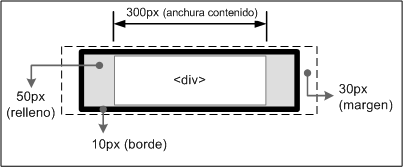
\includegraphics[width=0.75\textwidth]{figs/f0414.png}
\end{figure}
\end{center}

De esta forma, la anchura del elemento en pantalla sería igual a la suma de la anchura original, los márgenes, los bordes y los rellenos:

30px + 10px + 50px + 300px + 50px + 10px + 30px = 480 píxel

\end{frame}

%%---------------------------------------------------------------

\begin{frame}
\frametitle{Visualización}

\begin{itemize}
  \item CSS define otros cuatro atributos para controlar su visualización: display, visibility, overflow y z-index.
  \item El atributo display permite ocultar completamente un elemento haciendo que desaparezca de la página. Como el elemento oculto no se muestra, el resto de elementos de la página se mueven para ocupar su lugar.
  \item El atributo display también permite modificar el comportamiento de un elemento a bloque (block) o en línea (inline).
  \item El atributo visibility permite hacer invisible un elemento, lo que significa que el navegador crea la caja del elemento pero no la muestra. En este caso, el resto de elementos de la página no modifican su posición, ya que aunque la caja no se ve, sigue ocupando sitio.
\end{itemize}

\end{frame}



%%---------------------------------------------------------------

\begin{frame}
\frametitle{Diferencias entre display y visibility}

\begin{center}
\begin{figure}[p]
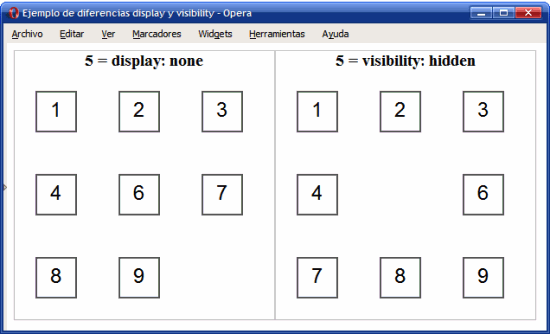
\includegraphics[width=0.8\textwidth]{figs/f0522.png}
\end{figure}
\end{center}

\end{frame}





%%---------------------------------------------------------------
%%---------------------------------------------------------------
\end{document}
%%---------------------------------------------------------------
%%---------------------------------------------------------------





%%---------------------------------------------------------------

\begin{frame}
\frametitle{Atributos margin}

\begin{center}
  \begin{table}
   \begin{tabular}{p{1.8cm}p{7.8cm}}
Atributos &\bf{margin-top}, \bf{margin-right}, \bf{margin-bottom}, \bf{margin-left} \\ \hline
Valores & $<medida>$ | $<porcentaje>$ | auto | inherit \\ \hline
Se aplica a & Todos los elementos, salvo margin-top y margin-bottom que sólo se aplican a los elementos de bloque y a las imágenes \\ \hline
Valor inicial & 0 \\ \hline
Descripción & Establece cada uno de los márgenes horizontales y verticales de un elemento \\  \hline
  \end{tabular}
    \caption{Definición del atributo \emph{margin-top}, \emph{margin-right}, \emph{margin-bottom}, \emph{margin-left} de CSS}
 \end{table}
\end{center}

\end{frame}

%%---------------------------------------------------------------

\begin{frame}
\frametitle{Atributo margin (atributo \emph{shorthand})}

\begin{center}
  \begin{table}
   \begin{tabular}{p{1.8cm}p{7.8cm}}
Atributo &\bf{margin} \\ \hline
Valores & ( $<medida>$ | $<porcentaje>$ | auto ) {1, 4} | inherit \\ \hline
Se aplica a & Todos los elementos salvo algunos casos especiales de elementos mostrados como tablas \\ \hline
Valor inicial & - \\ \hline
Descripción & Establece de forma directa todos los márgenes de un elemento \\ \hline
 \end{tabular}
   \caption{Definición del atributo margin de CSS}
 \end{table}
\end{center}

\end{frame}

%%---------------------------------------------------------------

\begin{frame}
\frametitle{Atributo margin (atributo \emph{shorthand}) (y II)}

La notación {1, 4} de la definición anterior significa que el atributo margin admite entre uno y cuatro valores, con el siguiente significado:

\begin{itemize}
  \item Si solo se indica un valor, todos los márgenes tienen ese valor.
  \item Si se indican dos valores, el primero se asigna al margen superior e inferior y el segundo se asigna a los márgenes izquierdo y derecho.
  \item Si se indican tres valores, el primero se asigna al margen superior, el tercero se asigna al margen inferior y el segundo valor se asigna los márgenes izquierdo y derecho.
  \item Si se indican los cuatro valores, el orden de asignación es: margen superior, margen derecho, margen inferior y margen izquierdo.
\end{itemize}

\end{frame}



\end {document}
